\section{Equilibrium}

\subsection{mechanical equilibrium}

equilibrium means no translational or rotational acceleration

equilibrium conditions are: $\boxed{\sum F = 0}$ and $\boxed{\sum \tau = 0}$

no resultant force: net force in any direction cancels out

no resultant torque: clockwise and anti-clockwise torques cancel out about any point

for a system of objects, one can take any single object or treat entire system as a whole

when treating individual objects, should consider internal forces between one and another

note internal forces always come in pairs (Newton’s 3$^\text{rd}$ law, action-reaction principle)

when treating whole system, only external forces are important

\subsection{frictional forces}

static friction is a self-adjustive force that always opposes trend of relative motion

maximum static friction depends on roughness of surface and strength of contact force

empirical rule states that $\boxed{f \leq f_\text{lim} = \mu N}$ , where $f_\text{lim}$ is called limiting friction

$\mu$ is called coefficient of friction, rough surfaces have larger values of $\mu$

for equilibrium, i.e., object does not slide over surfaces, one requires $\boxed{\mu \geq \frac{f}{N}}$

\subsubsection*{tips for solving equilibrium problems}

\begin{compactitem}
	\item when you encounter a force of unknown magnitude acting at some bizarre angle (force at a hinge or a rough peg, tension at end of a beam, etc.), taking moments about where this force acts might be a good idea to get around it
	
	\item for a system with several mutually interacting objects, write down equilibrium equations for the system as a whole might lead to a breakthrough
	
	\item sometimes you need to solve a set of simultaneous equations to determine one particular force, when you find any one of your equation does not work out, just stay patient and try a few more
	
	\item last but not least, don't panic, you have all the freedom to try to write down a whole set of equations, some of them will eventually work out
\end{compactitem}

\example{a uniform rod $AC$ of length $8a$ and weight W rests in equilibrium against surface of a smooth cylinder, which is against a vertical wall. The rod is inclined at an angle $\theta$ to a rough horizontal plane, where $\cos\theta=\frac{3}{5}$. A particle of weight $kW$ is attached to the rod at $C$. Given that $AB = 5a$, and the value of coefficient of friction between the rod and the ground is $\mu = \frac{3}{4}$. Find the set of values of $k$ for which equilibrium is possible.} \label{ex-rodball}

\begin{figure}[htp]
	\begin{center}
		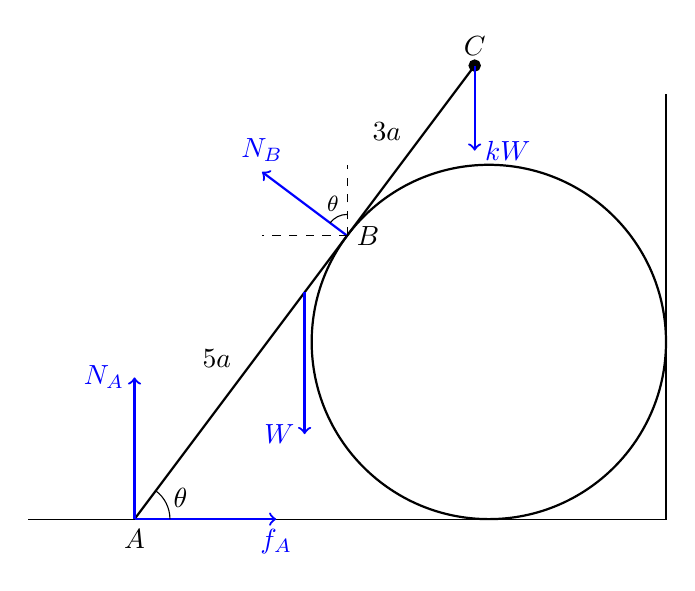
\begin{tikzpicture}[scale=0.9]
		\draw[thick] (0,0) circle (2.5);
		\draw[thick] (-5,-2.5) node[below] {$A$} --++ (4.8,6.4);
		\draw (-6.5,-2.5) --++ (9,0) --++ (0,6);
		\draw[fill] (-0.2,3.9) circle(0.08) node[above] {$C$};
		\draw[thick,blue,->] (-5,-2.5) --++ (0,2) node[left]{$N_A$};
		\draw[thick,blue,->] (-5,-2.5) --++ (2,0) node[below]{$f_A$};
		\draw[thick,blue,->] (-2,1.5) --++ (-1.2,0.9) node[above]{$N_B$};
		\draw[thick,blue,->] (-2.6,0.7) --++ (0,-2) node[left]{$W$};
		\draw[thick,blue,->] (-.2,3.9) --++ (0,-1.2) node[right]{$kW$};
		\draw (-4.5,-2.5) arc(0:53.13:0.5);
		\node at (-4.35,-2.2) {$\theta$};
		\node[right] at (-2,1.5) {$B$};
		\node[above left] at (-3.5,-0.5) {$5a$};
		\node[above left] at (-1.1,2.7) {$3a$};
		\draw[dashed] (-2,1.5) --++ (-1.2,0);
		\draw[dashed] (-2,1.5) --++ (0,1);
		\draw (-2,1.8) arc(90:143.13:0.3);
		\node at (-2.2,1.95) {{\footnotesize $\theta$}};
		\end{tikzpicture}
%		
%		Example \ref{ex-rodball}
	\end{center}
\end{figure}

\vspace*{-1\baselineskip}

take moments about $A$:

{
	
	\centering
	
	$N_B \cdot 5a = W \cdot 4a\cos\theta + kW \cdot 8a \cos\theta$
	
	$5N_B = 4\cdot\frac{3}{5}W + 8\cdot\frac{3}{5}kW \RA N_B = \frac{12+24k}{25}W$
	
}

resolve horizontally:

{
	
	\centering
	
	$f_A = N_B\sin\theta \RA f_A = \frac{12+24k}{25}W \times \frac{4}{5} \RA f_A = \frac{48+96k}{125}W$
	
}

resolve vertically:

{
	
	\centering
	
	$N_A + N_B \cos\theta = W + kW \RA N_A = W+kW -\frac{12+24k}{25}W \cdot \frac{3}{5} \RA N_A = \frac{89+53k}{125}W$
	
}

no sliding between rod and ground requires:

{
	
	\centering
	
	$f_A\leq \mu N_A \RA \frac{48+96k}{125}W \leq \frac{3}{4}\times \frac{89+53k}{125}W \RA 4(48+96k) \leq 3(89+53k)$
	
	$\RA 192 + 384k \leq 267 + 159k \RA 225k \leq 75 \RA k\leq \frac{1}{3}$
	
}

so range for values of $k$ is $0<k\leq \frac{1}{3}$ \eoe

\newpage

\vspace*{-1.2\baselineskip}

\example{Two uniform rods $AB$ and $AC$ are smoothly hinged at $A$. Rod $AB$ has length $8a$ and weight $3W$. Rod $AC$ has length $6a$ and weight $2W$. The rods are in equilibrium in a vertical plane with $B$ and $C$ resting on a rough horizontal plane and angle $CAB$ forms a right angle. (a) Find the force between the two rods at the hinge $A$. (b) The coefficient of friction between each rod and the floor is $\mu$. Find the least possible value of $\mu$.} \label{ex-tworods}

\begin{figure}[htp]
	\begin{center}
		\begin{tikzpicture}[scale=1]
		\draw (-2,0) -- (12,0);
		\draw[thick] (0,0) node[below]{$B$} -- (3.2,2.4) node[midway,above left]{$4a$} -- (6.4,4.8) node[above]{$A$} node[midway, above left]{$4a$} -- (8.2,2.4) node[midway,above right]{$3a$} -- (10,0) node[below]{$C$} node[midway,above right]{$3a$};
		\draw[thick,blue,->] (3.2,2.4) --++ (0,-1.5) node[right]{$3W$};
		\draw[thick,blue,->] (8.2,2.4) --++ (0,-1) node[left]{$2W$};
		\draw[thick,blue,->] (0,0) --++ (1.5,0) node[below]{$f_B$};
		\draw[thick,blue,->] (0,0) --++ (0,1.5) node[left]{$N_B$};
		\draw[thick,blue,->] (10,0) --++ (-1.5,0) node[below]{$f_C$};
		\draw[thick,blue,->] (10,0) --++ (0,1.5) node[right]{$N_C$};
		\draw[thick,blue,->] (6.3,4.8) --++ (-0.8,1.6) node[left]{$F_A$};
		\draw[thick,blue,->] (6.4,4.7) --++ (0.8,-1.6) node[left]{$F_A$};
		\end{tikzpicture}
%		
%		Example \ref{ex-tworods}
	\end{center}
\end{figure}

\vspace*{-1\baselineskip}

take moments about $C$ for system:

{

\centering

$3W\cdot\left(4a\cos\theta+6a\sin\theta\right)+2W\cdot(3a\sin\theta)=N_B\cdot 10a$

$3W\cdot(4a\times\frac{4}{5}+6a\times\frac{3}{5})+2W\cdot(3a\times\frac{3}{5}) = N_B \cdot 10a$

$10 N_B = \left(\frac{48}{5} + \frac{54}{5} + \frac{18}{5}  \right) = 24 W \RA N_B = \frac{12}{5}W$

} 

take moments about $A$ for rod $AB$:

{
	
\centering
	
$N_B\cdot 8a\cos\theta = 3W\cdot 4a\cos\theta + f_B \cdot 8a\sin\theta$

$\frac{12}{5}W \cdot 8a\cdot\frac{4}{5} = 3W \cdot 4a\cdot\frac{4}{5} + f_B \cdot 8a\cdot\frac{3}{5}$

$\frac{96}{5}W = 12W + 6f_B \RA f_B = \frac{6}{5}W$
	
}

resolve horizontally for rod $AB$:

{
	
\centering
	
$F_{A,x} = f_B \RA F_{A,x} = \frac{6}{5}W$
	
}

resolve vertically for rod $AB$:

{
	
\centering
	
$N_B + F_{A,y} = 3W \RA F_{A,y} = 3W - \frac{12}{5}W = \frac{13}{5}W$
	
}

hence we find interaction at hinge $A$:

{
	
\centering
	
$F_A = \sqrt{F_{A,x}^2 + F_{A,y}^2} = \sqrt{\left(\frac{6}{5}W\right)^2 + \left(\frac{13}{5}W\right)^2} \RA F_A = \frac{\sqrt{205}}{5}W$
	
}

resolve horizontally for system:

{
	
\centering
	
$f_C = f_B \RA f_C = \frac{6}{5}W$
	
}

resolve vertically for system:

{
	
\centering
	
$N_B + N_C = 3W + 2W \RA N_C = 5W - \frac{12}{5}W \RA N_C = \frac{13}{5}W$
	
}

at contact $B$ and $C$, using $\mu \geq \frac{f}{N}$

{
	
\centering

$\mu_B \geq \frac{\frac{6}{5}W}{\frac{12}{5}W}=\frac{1}{2} \quad$ and $\quad$ $\mu_B \geq \frac{\frac{6}{5}W}{\frac{13}{5}W}=\frac{6}{13}$

}

no sliding at either $B$ or $C$ requires $\mu \geq \tmax(\mu_B, \mu_C)$, so $\mu \geq \frac{6}{13}$ \eoe

%\newpage
%
%\vspace*{-\baselineskip}

\example{A uniform rod $AB$ of weight $W$ and length $2a$ rests on a rough horizontal plane. A light inextensible string $BC$ is attached to the rod at $B$ and passes over a small smooth fixed peg $P$, which is at a distance $3a$ vertically above end $A$. A particle of weight $kW$ is attached at $C$ and hangs vertically. $A$, $B$ and $C$ are in the same vertical plane. In equilibrium the rod is inclined at an angle $\theta$ to the
horizontal where $\sin\theta=\frac{3}{5}$. (a) Given that the system is in limiting equilibrium, find the coefficient of friction between the rod and the plane is $\mu$. (B) Find the value of $k$.}

\begin{figure}[htp]
	\begin{center}
		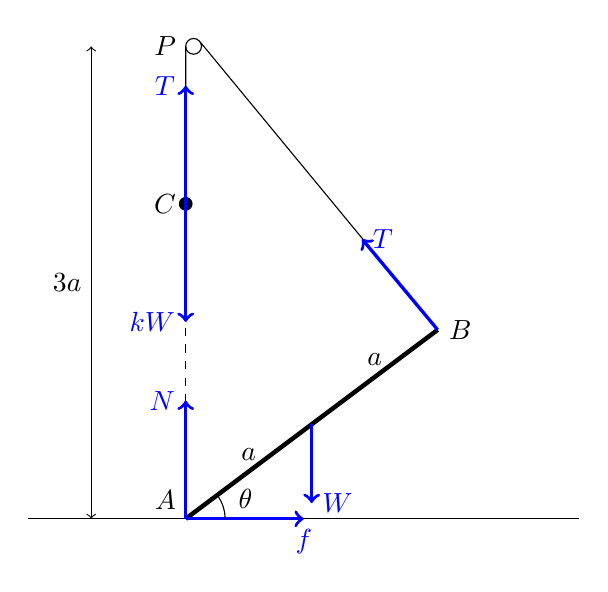
\begin{tikzpicture}[scale=1]
		\draw (-2,0) -- (5,0);
		\draw[dashed] (0,0) node[above left]{$A$} -- (0,6) node[left]{$P$};
		\draw[fill] (0,4) circle(0.08) node[left]{$C$} -- (0,6);
		\draw[ultra thick] (0,0) -- (1.6,1.2) node[midway,above]{$a$} -- (3.2,2.4) node[right]{$B$} node[midway,above]{$a$};
		\draw (0.1,6) circle(0.1) ++ (42:0.1) -- (3.2,2.4);
		\draw[very thick,blue,->] (0,0) --++ (1.5,0) node[below]{$f$};
		\draw[very thick,blue,->] (0,0) --++ (0,1.5) node[left]{$N$};
		\draw[very thick,blue,->] (1.6,1.2) --++ (0,-1) node[right]{$W$};
		\draw[very thick,blue,->] (3.2,2.4) --++ (129.8:1.5) node[right]{$T$};
		\draw[very thick,blue,->] (0,4) --++ (0,-1.5) node[left]{$kW$};
		\draw[very thick,blue,->] (0,4) --++ (0,1.5) node[left]{$T$};
		\draw (0.5,0) arc(0:36.87:0.5);
		\node at (18:0.8) {$\theta$};
		\draw[<->] (-1.2,0) --++ (0,6) node[left,midway]{$3a$};
		\end{tikzpicture}
	\end{center}
\end{figure}

\vspace*{-1\baselineskip}

take moments about $P$ for the rod:

{

\centering

$f\cdot3a = W\cdot a\cos\theta \RA f=\frac{1}{3}W\cos\theta = \frac{1}{3}W\cdot\frac{4}{5} \RA f=\frac{4}{15}W$

}

take moments about $B$ for the rod:

{

\centering

$N\cdot2a\cos\theta = f\cdot2a\sin\theta + W\cdot a\cos\theta$

$2N\cdot\frac{4}{5} = 2\cdot\frac{4}{15}W\cdot\frac{3}{5} + W\cdot\frac{4}{5} \RA N=\frac{7}{10}W$

}

limiting friction so $\mu = \frac{f}{N} = \frac{4}{15} \cdot \frac{10}{7} \RA \mu = \frac{8}{21}$

resolve horizontally for rod: $T_x = f \RA T_x = \frac{4}{15}W$

resolve vertically for rod: $T_y + N = W \RA T_y = W - \frac{7}{10}W \RA T_y = \frac{3}{10}W$

tension in string is: $T = \sqrt{T_x^2+T_y^2} = \sqrt{\left(\frac{4}{15}\right)^2 + \left(\frac{3}{10}\right)^2} \cdot W \RA T=\frac{\sqrt{145}}{30}W$

equilibrium for particle $C$ requires $T=kW$, so $k=\frac{\sqrt{145}}{30}$ \eoe